
% JuliaCon proceedings template
\documentclass{juliacon}
\setcounter{page}{1}

\begin{document}

\input{header}

\maketitle

\begin{abstract}

MPI.jl is a Julia package for using the Message Passing Interface (MPI),
a standardized and widely-supported communication interface for
distributed computing, with multiple open source and proprietary
implementions. It roughly follows the C MPI interface, with some
additional conveniences afforded by the Julia language such as automatic
handling of buffer lengths and datatypes.

\end{abstract}

\section{Introduction}

Now over 25 years old, MPI is the stalwart of high-performance computing
communication, supported on everything from single machines to
billion-dollar supercomputers. Despite its age, it supports several
models of communication, and significant engineering effort goes into
optimizing performance and supporting the latest networking hardware.

Although Julia provides its own suite of distibuted computing tools via
the Distributed standard library, it is based on a controller/worker
model and is currently unable to leverage fast networking hardware such
as InfiniBand, which limits its scalability to large problems. MPI.jl
leverages the well-established and proven technology, including
extensions such as the CUDA-aware interfaces for multi-GPU
communication. It is being used by multiple Julia projects, including
the CliMA Earth system modelling project \cite{clima}.

\subsection{History}

MPI.jl originated as a repository developed by Lucas Wilcox in July 2012, 4 months after
Julia was first publicly announced. It was registered in the Julia package registry in
2014, and since then has evolved considerably along with the Julia language itself. It has
so far received contributions from 51 people: many of these are users who required the
addition of a specific piece of functionality.

Major changes to the codebase were typically precipitated by changes in the Julia language
itself, modifications to the build system to support different MPI implementations (see
section \ref{sec:application-binary-interface}) or addition of support for new
platforms. The interface has stayed remarkably consistent over time, the only major change
at the highest level being the recent addition of buffer types (section
\ref{sec:buffers-datatypes-and-operators}).

\section{Simple example and running MPI programs}
\label{sec:simple-example}

Most MPI programs utilise a single-program, multiple-data (SPMD) model
where multiple processes all run the same program and communicate via
messages, with their data determined by the process rank (a 0-based
ordering of the processes).

An example of this is a simple ``round-robin'' communication pattern
in which each process sends a message containing its rank to its next
neighbor using nonblocking point-to-point operations:

\begin{lstlisting}[language = Julia]
# sendrecv.jl
# initialize and set global variables
using MPI
MPI.Init()

comm = MPI.COMM_WORLD
rank = MPI.Comm_rank(comm)
N = MPI.Comm_size(comm)

# nonblocking receive from previous rank
recv_buf = Array{Float64}(undef, 2)
recv_req = MPI.Irecv!(recv_buf, mod(rank-1, N), 0,
                      comm)

# nonblocking send to next rank
send_buf = Float64[rank, rank]
send_req = MPI.Isend(send_buf, mod(rank+1, N), 0,
                     comm)

# block until communication is completed
MPI.Waitall!([recv_req, send_req])
print("$rank: Received $recv_buf\n")
\end{lstlisting}

This can be run using the MPI launcher, typically called
\verb mpiexec :

\begin{verbatim}
$ mpiexec -n 3 julia sendrecv.jl
0: Received [2.0, 2.0]
2: Received [1.0, 1.0]
1: Received [0.0, 0.0]
\end{verbatim}

\section{Implementation details and challenges}
\label{sec:implementation-details-and-challenges}

Although MPI.jl mirrors the C MPI interface quite closely, it does take advantage of
several features of the Julia language to improve usability. Many of these changes were
heavily influenced by the mpi4py package \cite{dalcin2011parallel} which provides MPI
bindings for Python, and has a similar aim of making MPI functionality easily useable in a
high-level, dynamic language.

The C and Fortran MPI interfaces require that users manually
check the error code returned by each function; MPI.jl is able to use
Julia's exception handling machinery to automatically check error codes
and print readable error messages. This allows functions to return their
results via return values instead of via additional functions arguments.
For example, nonblocking operations return \verb Request  objects;
blocking receive operations return their output buffers.

\subsection{Functionality}

Most commonly-used MPI functionality is currently available via the package, including
dynamic process management and operations for point-to-point (blocking and nonblocking),
collective, one-sided and I/O.

The MPI 3.1 standard lists several hundred functions: limited maintainer resources means
that the addition of features is mainly driven by needs of the contributors and requests
by users, and so lesser-used MPI features are not yet available. This includes
neighbourhood and non-blocking collectives, persistent operations,
buffered/synchronous/ready point-to-point operations.

\subsection{Allocation and serialization}
\label{sec:allocation-and-serialization}

For communication operations which receive data, MPI.jl typically
defines two separate functions:

\begin{itemize}
\item
  one function in which the output buffer is supplied by the user: as it
  mutates this value, it adopts the Julia convention of suffixing with
  \verb !  (e.g.~\verb MPI.Recv! , \verb MPI.Reduce! ).
\item
  one function which allocates the buffer for the output
  (\verb MPI.Recv , \verb MPI.Reduce ).
\end{itemize}

Additionally, we adopt the convention from mpi4py of using lowercase names for
functions which are able to handle arbitrary objects. These are typically
slower as they rely on serialization and are not type-stable, but can be
convenient as they don't require that the object type or size be known
by the receiver. Currently only a small number of these functions are
provided.

\subsection{Buffers, datatypes and operators}
\label{sec:buffers-datatypes-and-operators}

In C and Fortran, MPI communication functions require three arguments
(address, count and element datatype) to specify their input and/or
output buffers e.g.~the \verb MPI_Send  signature in C has six
arguments:
\begin{lstlisting}[language = C]
int MPI_Send(const void* buf, int count,
      MPI_Datatype datatype, int dest, int tag,
      MPI_Comm comm)
\end{lstlisting}

In Julia, these can all be determined from an \verb Array  object, so
the corresponding function in MPI.jl only requires 4 arguments:
\begin{lstlisting}[language = Julia]
MPI.Send(buf, dest::Integer, tag::Integer,
      comm::MPI.Comm)
\end{lstlisting}

An intermediate \verb Buffer  type is defined that captures the pointer, length and
datatype properties, and allows defining MPI communication operations for other Julia
objects without requiring that additional methods for every communication function. For
example, to support the CUDA-aware MPI interface across all MPI functions, only a small
number of interface functions were required at the buffer level.

Additional ``chunked'' buffer types are defined for collective operations which split the
buffer among multiple processes in a communicator. For example, the \verb UBuffer (an
abbreviation for ``uniformly chunked'') is used as the send buffer for \verb MPI.Scatter!  or
the receive buffer for \verb MPI.Gather! ; similarly the \verb VBuffer (``variable-length buffer'')
is used for \verb MPI.Scatterv!  and \verb MPI.Gatherv! .

For contiguous arrays the buffer will determine the default MPI datatype based on the
element type of the underlying array: for standard integer, floating point and complex
number types, MPI.jl will use the predefined MPI datatypes. For other Julia bitstypes
(primitive types or immutable structs with fields that are also bitstypes), or if the
buffer is a strided view, MPI.jl will build and commit a corresponding MPI user-defined
type. A lower-level, C-like interface for manually constructing and committing MPI
datatypes is also available.

Similarly, for MPI collective reduction operations (\verb MPI.Reduce , \verb MPI.Scan ,
etc.), MPI.jl will convert Julia functions to MPI operator objects, either mapping to
predefined operators (e.g.~\verb +  to \verb MPI.SUM ), or wrapping functions to form
custom operators.

The pooled variance example in section \ref{sec:pooled-variance} illustrates the use of
both custom datatypes and custom operators.

\subsection{Application binary interface}
\label{sec:application-binary-interface}

The MPI standard specifies C and Fortran appilication programming
interfaces (API), but not an application binary interface (ABI).
Consequently, datatypes and enum values vary between different
implementations, and require parsing C headers to extract their precise
values. After much experimentation, we have settled on two approaches that
work reasonably well and require minimal user intervention:

\begin{itemize}
\item
  Attempt to identify the MPI implementation by querying
  \verb MPI_Get_library_version , and use predefined constants and
  types if known to be compatible with MPICH, Open MPI or Microsoft MPI.
  This should cover most MPI implementations released since the completion of the
  MPICH ABI compatibility initiative in 2016.
\item
  Otherwise, at build time it compiles a small C program that outputs
  the type sizes and constants. One complication is that the opaque C
  handles might only be defined at link time: in this case, we convert
  to the Fortran handle values (which are required to be integers), and
  convert back to C handles when calling \verb MPI.Init() . A similar
  approach is used by the MPI bindings for Rust \cite{rsmpi}.
\end{itemize}

\subsection{Binary support}
\label{sec:binary-support}

Similar to many Julia packages, MPI.jl uses BinaryBuilder and the
Artifacts system to automatically install an MPI implementation when the
package is installed (currently Microsoft MPI on Windows, MPICH on other
platforms). This completely automates the installation procedure for users on
single machines, meaning that MPI.jl can be added as a project dependency without
users being required to correctly install their own MPI implementation.

On high-performance computing systems one would typically want to use system or other
externally-provided binaries. To aid this, MPI.jl provides additional hooks to enable
switching this at build time via environment variables, and a warning is shown if a user
appears to be using the default MPI binary on a HPC cluster. Challenges remain on how to
make it easier to switch implementations, such as how to correctly invalidate the package
precompilation cache.

There are similar challenges when working with external libraries which also depend on
MPI, such as HDF5 and PETSc. For example, HDF5.jl has recently added MPI support, but it
requires that the user provide their own HDF5 library that has been correctly linked
against the same MPI library used by MPI.jl. This makes it difficult to distribute Julia
packages that make use of such functionality. We are investigating ways to improve this,
such as integration with the Spack package manager \cite{spack}.

\subsection{Combining with other modes of Julia parallelism}

Julia itself provides three models of parallelism: asynchronous tasks/coroutines (green
threading), simultaneous multi-threading and distributed computing.

Though MPI nonblocking operations act in a similar manner to tasks, they can't be
integrated directly with Julia's runtime scheduler as MPI does not provide a mechanism to
interact with the Julia event loop. Furthermore, calls from Julia to external libraries
will block the event loop, which means that calling a blocking MPI operations in a
separate task will not yield until it completes.  One simple but inefficient approach is
to use a spinloop with a call to a non-blocking query operation:
\begin{lstlisting}[language = Julia]
mpitask = @async begin
  done = false
  while !done
    done, _ = MPI.Test!(request)
    yield()
  end
end

aftertask = @async begin
  wait(mpitask)
  # code to run after MPI communication complete
end

wait(aftertask)
\end{lstlisting}

If the MPI library is initialized with multi-threading support via \verb MPI.Init_thread ,
then MPI.jl functions can safely be called from Julia tasks scheduled on different
threads. For example, the above spinloop could be replaced by
\begin{lstlisting}[language = Julia]
mpitask = Threads.@spawn MPI.Wait!(request)
\end{lstlisting}
however concurrency will be limited by the available threads.

Julia's Distributed standard library is based on remote procedure calls. The
MPIClusterManagers.jl package builds on MPI.jl to allow both MPI and Distributed
operations, as well as use of MPI as a communication protocol for Distributed.

One useful feature of the Distributed library is that it enables interactive distributed
computing through a REPL or notebook interface. Unfortunately attempts to provide similar
functionality for MPI.jl have so far had limited success. The input and output redirection
imposed by the MPI launchers make it difficult to run MPI sessions interactively.

Most common MPI implementations support ``singleton'' initialization where a single
process started outside a launcher can call \verb MPI_Init . This is widely used by Julia
projects which support both interactive serial and batch parallel functionality. Though
the MPI standard encourages implementations to allow such singleton processes to connect
with each other, we have yet to find any implementations which support such operation.


\section{Examples}
\label{sec:examples}

\subsection{Ping pong benchmark}
\label{sec:ping-pong-benchmark}

The ``ping pong'' benchmark consists of two MPI processes which
alternate sending messages between each other, and is a useful measure
of how function call overhead affects communication latency.

A simple Julia implementation is:
\begin{lstlisting}[language = Julia]
function pingpong(T, bufsize, iters)
    buffer = zeros(T, bufsize)
    comm = MPI.COMM_WORLD
    rank = MPI.Comm_rank(comm)
    tag = 0

    MPI.Barrier(MPI.COMM_WORLD)
    tic = MPI.Wtime()
    for i = 1:iters
        if rank == 0
            MPI.Send(buffer, 1, tag, comm)
            MPI.Recv!(buffer, 1, tag, comm)
        else
            MPI.Recv!(buffer, 0, tag, comm)
            MPI.Send(buffer, 0, tag, comm)
        end
    end
    toc = MPI.Wtime()

    avgtime = (toc-tic)/iters
    return avgtime
end
\end{lstlisting}


\begin{figure}[t]
\centerline{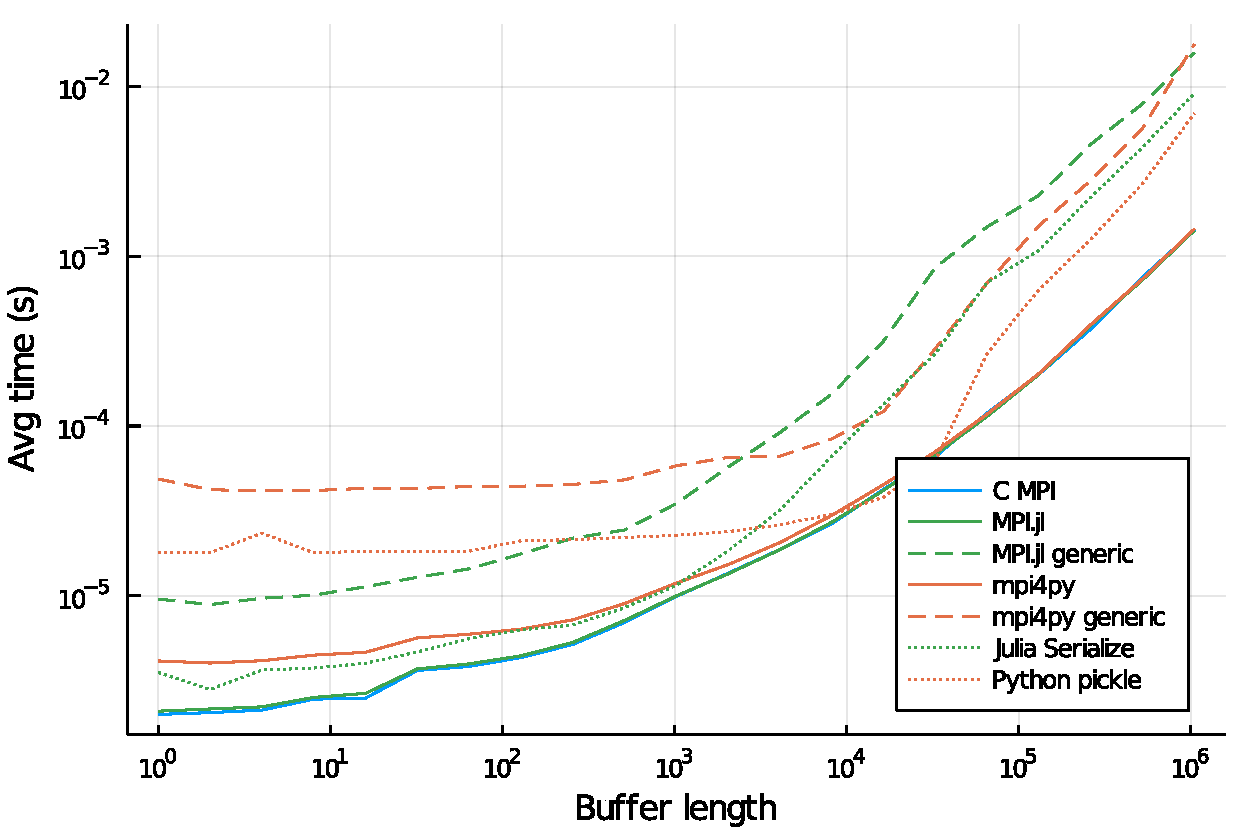
\includegraphics[width=0.5\textwidth]{pingpong.pdf}}
\caption{MPI ping pong benchmark in C, Julia (MPI.jl) and Python (mpi4py) using arrays of
  64-bit floating-point numbers. For reference, the cost of serializing and deserializing
  an array (Serialization in Julia, pickle in Python) are also shown.
  Benchmarks were performed using Open MPI 4.0.4, using two processes on different nodes
  connected by EDR InfiniBand, Julia 1.5.2 with MPI.jl 0.15.1, and Python 3.8.5 with
  mpi4py 3.0.3.
  \label{fig:pingpong}}
\end{figure}

Figure \ref{fig:pingpong} compares the ping pong benchmark implemented in
C, Julia using MPI.jl, and Python using mpi4py. The MPI.jl benchmark
exhibits similar performance to C, whereas mpi4py is notable slower for
smaller message sizes, likely due to the intepreter overhead of Python.

In addition, for MPI.jl and mpi4py we also compare the lowercase
``generic'' \verb MPI.send  and \verb MPI.recv  functions, which are able to
handle arbitrary objects. Here MPI.jl is still faster than mpi4py for
small messages, but slower for medium-sized messages. This appears to largely
be determined by the relative performance of the serialization in each language.

\subsection{Minimum-spanning tree broadcast}
\label{sec:minimum-spanning-tree-broadcast}

Julia syntax is close to pseudo-code found in the literature to describe
parallel algorithms. For example, consider the minimum-spanning tree
broadcast algorithm in Figure 3a of \cite{chan2007collective}. A Julia
implementation is given as:

\begin{lstlisting}[language = Julia]
function MSTBcast(x, root, left, right, comm)
    me = MPI.Comm_rank(comm)
    tag = 999

    if left == right
        return x
    end
    mid = div((left + right),  2)
    dest = root <= mid ? right : left

    if me == root
        MPI.send(x, dest, tag, comm)
    end
    if me == dest
        (x, _) = MPI.recv(root, tag, comm)
    end

    if me <= mid && root <= mid
        MSTBcast(x, root, left, mid, comm)
    elseif me <= mid && root > mid
        MSTBcast(x, dest, left, mid, comm)
    elseif me > mid && root <= mid
        MSTBcast(x, dest, mid + 1, right, comm)
    elseif me > mid && root > mid
        MSTBcast(x, root, mid + 1, right, comm)
    end
end
\end{lstlisting}

This is nearly identical to the pseudo-code and can be called for all of
the datatypes supported by \verb MPI.send  and \verb MPI.recv , for
example arrays, functions, and dictionaries.

\subsection{Pooled variance using custom datatypes and operators}
\label{sec:pooled-variance}

Computing the variance of a distributed array $x$ illustrates the power of custom datatypes
and reduction operations. Using the standard formula
\[
  \mathrm{Var}(x) = \frac{1}{n} \sum_{i=1}^n (x_i - \bar x)^2
\]
requires two rounds of communication (first to sum $x_i$ and broadcast the mean, second to sum the squared differences). Using the sum-of-squares formula
\[
  \mathrm{Var}(x) = \frac{1}{n} \sum_{i=1}^n x_i^2 - \bar x^2
\]
can be done in one communication operation (by summing both $x_i^2$ and $x_i$), but suffers from numerical cancellation error. The pooled variance formula is a numerically stable way of computing the variance of $x$ from the means and variances of a partitioning $(x^{(k)})_{k=1}^K$ of $x$:
\[
  \mathrm{Var}(x) = \sum_k \frac{n^{(k)}}{n} \left[ \mathrm{Var}(x^{(k)}) + \bar x^{(k)} (\bar x^{(k)} - \bar x) \right]
\]
This can applied recursively as a custom reduction operator on objects containing the mean, variance and length of each element of the partition, requiring only a single \verb MPI.Reduce  operation:

\begin{lstlisting}[language = Julia]
# Custom struct containing the summary statistics
struct SummaryStat
    mean::Float64
    var::Float64
    n::Float64
end

function SummaryStat(X::AbstractArray)
    m = mean(X)
    v = varm(X,m,corrected=false)
    n = length(X)
    SummaryStat(m,v,n)
end

# Custom reduction operator, computing pooled mean,
# variance and length
function pool(S1::SummaryStat, S2::SummaryStat)
    n = S1.n + S2.n
    m = (S1.mean * S1.n + S2.mean * S2.n) / n
    v = (S1.n * (S1.var + S1.mean * (S1.mean-m)) +
         S2.n * (S2.var + S2.mean * (S2.mean-m))
        ) / n
    SummaryStat(m,v,n)
end

# Perform a scalar reduction to `root`
summ = MPI.Reduce(SummaryStat(X), pool, root, comm)
\end{lstlisting}

\section{Acknowledgements}
\label{sec:acknowledgements}

We thank the many contributors to MPI.jl over the years: Erik Schnetter,
Jared Crean, Jake Bolewski, Davide Lasagna, Katharine Hyatt, Jeremy
Kozdon, Andreas Noack, Bart Janssens, Amit Murthy, Steven G. Johnson,
David Anthoff, Thomas Bolemann, Joey Huchette, Seyoon Ko, Juan Ignacio
Polanco, Tristan Konolige, Samuel Omlin, Mosè Giordano, Filippo
Vicentini, Keno Fischer, Maurizio Tomasi, Yuichi Motoyama, Tom Abel,
Jane Herriman, Ernesto Vargas, Elliot Saba, Rohan McLure, Randy Lai,
Mike Nolta, Josh Milthorpe, Michel Schanen, Kiran Pamnany, Joaquim Dias
Garcia, Jonathan Goldfarb, Chris Hill, Balazs Nemeth, Alberto F. Martin,
Ali Ramadhan, Viral Shah, Sacha Verweij, Kristoffer Carlsson, Joel Mason
and Yao Lu.

This research was made possible by the generosity of Eric and Wendy
Schmidt by recommendation of the Schmidt Futures program, Mountain
Philanthropies, the Paul G. Allen Family Foundation, and the National
Science Foundation (NSF award AGS-1835860).

\bibliographystyle{juliacon}
\bibliography{paper}

\end{document}

% Inspired by the International Journal of Computer Applications template
